 \documentclass [12pt]{article} 

\usepackage {amsmath}
\usepackage {amsthm}
\usepackage {amssymb}
\usepackage {graphicx} 
\usepackage {float}
\usepackage {multirow}
\usepackage {xcolor}
\usepackage {algorithmic}
\usepackage [ruled,vlined,commentsnumbered,titlenotnumbered]{algorithm2e} \usepackage {array} 
\usepackage {booktabs} 
\usepackage {url} 
\usepackage {parskip} 
\usepackage [margin=1in]{geometry} 
\usepackage [T1]{fontenc} 
\usepackage {cmbright} 
\usepackage [many]{tcolorbox} 
\usepackage [colorlinks = true,
            linkcolor = blue,
            urlcolor  = blue,
            citecolor = blue,
            anchorcolor = blue]{hyperref} 
\usepackage {enumitem} 
\usepackage {xparse} 
\usepackage {verbatim}
\usepackage{listings}
\usepackage{xcolor}
\lstset { %
    language=C++,
    backgroundcolor=\color{black!5}, % set backgroundcolor
    basicstyle=\footnotesize,% basic font setting
}
\newtheorem{theorem}{Theorem}
\newtheorem{remark}{Remark}
\newtheorem{lemma}[theorem]{Lemma}
\theoremstyle{definition}
\newtheorem{definition}{Definition}[section]
\newtheorem{claim}{Claim}




\DeclareTColorBox {Solution}{}{breakable, title={Solution}} \DeclareTColorBox {Solution*}{}{breakable, title={Solution (provided)}} \DeclareTColorBox {Instruction}{}{boxrule=0pt, boxsep=0pt, left=0.5em, right=0.5em, top=0.5em, bottom=0.5em, arc=0pt, toprule=1pt, bottomrule=1pt} \DeclareDocumentCommand {\Expecting }{+m}{\textbf {[We are expecting:} #1\textbf {]}} \DeclareDocumentCommand {\Points }{m}{\textbf {(#1 pt.)}} 

\begin {document} 

\vspace {1em} 
\begin {Instruction} 
Adapted From Virginia Williams' lecture notes.
\end {Instruction}  

{\LARGE \textbf {COMP 285 (NC A\&T, Spr `22)}\hfill \textbf {Lecture 22} } 

\begin{centering}
\section*{Single-Source Shortest Path in Weighted Graphs}
\end{centering}


\section{Dijkstra's Algorithm}

Now we will solve the single source shortest paths problem in graphs with nonnengative
weights using Dijkstra's algorithm. The key idea, that Dijkstra will maintain as an invariant,
is that $\forall t in V$, the algorithm computes an estimate $d[t]$ of the distance of $t$ from the source such that:

\begin{enumerate}
    \item At any point in time, $d[t] \geq d(s, t)$, and
    \item when t is finished, $d[t] = d(s, t)$.
\end{enumerate}


\begin{algorithm}
\caption{Dijkstra($G= (V,E), S$)}
\label{alg:1}
\begin{algorithmic}
\STATE $\forall t \in V, d[t] \gets \infty$ \texttt{// set initial distance estimates}
\STATE $d[s] \gets 0$
\STATE $F \gets \{v \mid \forall v \in V\}$ \texttt{// F is the set of nodes that are yet to achieve final distances estimates}
\STATE $D \gets \emptyset$ \texttt{// D will be the set of nodes that have achieved final distance estimates}
\WHILE{$F \neq \emptyset$}
    \STATE $x \gets$ elements in $F$ with minimum distance estimate
    \FOR{$(x,y) \in E$}
        \STATE $d[y] \gets \min\{d[y], d[x] + w(x,y)\}$ \texttt{// "relax" the estimate of y}
        \STATE \texttt{// to maintain paths: if} $d[y]$ \texttt{changes, then } $\pi(y) \gets x$
    \ENDFOR
    \STATE $F \gets F \setminus \{x\}$
    \STATE $D \gets D \cup \{x\}$
\ENDWHILE
\end{algorithmic}
\end{algorithm}

\begin{claim}[For every $u$, at any point of time $d(u) \geq d(s, u)$.]
\vspace{1em}
A formal proof of this claim proceeds by induction. In particular, one shows that at any point in time, if $d[u] < \infty$, then $d[u]$ is the weight of some path from $s$ to $t$. Thus at any point $d[u]$ is at least the weight of the shortest path, and hence $d[u] \geq d(s, u)$. As a base case, we know that $d[s] = 0 = d(s, s)$ and all other distance estimates are $+\infty$, so we know that the claim holds initially. Now, when $d[u]$ is changed to $d[x] + w(x, u)$ then (by the induction hypothesis) there is a path from $s$ to $x$ of weight $d[x]$ and an edge $(x, u)$ of weight $w(x, u)$. This means there is a path from $s$ to $u$ of weight $d[u] = d[x] + w(x, u)$. This implies that $d[u]$ is at least the weight of the shortest path $= d(s, u)$, and the induction argument is complete
\end{claim}


\begin{claim}[When node $x$ is placed in $D$, $d(x) = d(s,x)$] 
\vspace{1em}

Notice that proving the above claim is sufficient to prove the correctness of the algorithm since $d[x]$ is never changed again after $x$ is added to $D$: the only way it could be changed is if for some node $y \in F$ , $d[y] + w(y, x) < d[x]$ but this can't happen since $d[x] \leq d[y ]$ and $w(y, x) \geq 0$ (all edge weights are nonnegative). The assertion $d[x] \leq d[y]$ for all $y \in F$ stays true at all points after $x$ is inserted into D: assume for contradiction that at some point for some $y \in F$ we get $d[y ] < d[x]$ and let $y$ be the first such $y$ . $Before d[y ]$ was updated $d[y' ] \geq d[x]$ for all $y' \in F$ . But then when $d[y ]$ was changed, it was due to some neighbor $y'$ of $y$ in $F$ , but$ d[y' ] \geq d[x]$ and all weights are nonnegative, so we get a contradiction 

We prove this claim by induction on the order of placement of nodes into $D$. For the base case, $s$ is placed into D where $d[s] = d(s, s) = 0$, so initially, the claim holds. 

For the inductive step, we assume that for all nodes $y$ currently in $D$, $d[y ] = d(s, y )$. Let $x$ be the node that currently has the minimum distance estimate in $F$ (this is the node about to be moved from $F$ to $D$). We will show that $d[x] = d(s, x)$ and this will complete the induction. Let $p$ be a shortest path from $s$ to $x$. Suppose $z$ is the node on $p$ closest to $x$ for which $d[z] = d(s, z)$. We know $z$ exists since there is at least one such node, namely $s$, where $d[s] = d(s, s)$. By the choice of $z$, for every node $y$ on $p$ between $z$ (not inclusive) to $x$ (inclusive), $d[y ] > d(s, y )$. Consider the following options for $z$.

\begin{enumerate} 
    \item If $z = x$, then $d[x] = d(s, x)$ and we are done.
    \item Suppose $z \neq x$. Then there is a node $z'$ after $z$ on $p$. (Here it is possible that $z' = x$.) We know that $d[z] = d(s, z) \leq d(s, x) \leq d[x]$. The first $\leq$ inequality holds because subpaths of shortest paths are shortest paths as well, so that the prefix of $p$ from $s$ to $z$ has weight $d(s, z)$. In addition, the weights on edges are non-negative, so that the portion of $ p$ from $z$ to $x$ has a nonnegative weight, and so $d(s, z) \leq d(s, x)$. The subsequent $\leq $ holds by Claim 1. We know that if $d[z] = d[x]$ all of the previous inequalities are equalities and $d[x] = d(s, x)$ and the claim holds. 

    Finally, towards a contradiction, suppose $d[z] < d[x]$. By the choice of $x \in F$ we know $d[x]$ is the minimum distance estimate that was in $F$ . Thus, since $d[z] < d[x]$, we know $z \notin F$ and must be in $D$, the finished set. This means the edges out of $z$, and in particular ($z, z' )$, were already relaxed by our algorithm. But this means that $d[z ' ] \leq d(s, z) + w(z, z' ) = d(s, z' )$, because $z$ is on the shortest path from $s$ to $z '$ , and the distance estimate of $z '$ must be correct. However, this contradicts $z$ being the closest node on $p$ to $x$ meeting the criteria$ d[z] = d(s, z)$. Thus, our initial assumption that $d[z] < d[x]$ must be false and $d[x]$ must equal $d(s, x)$.
\end{enumerate}
\end{claim}


\subsection{Implementation of Dijkstra's Algorithm}

Consider implementing Dijkstra's algorithm with a priority queue to store the set $F$ , where the distance estimates are the keys. The initialization step takes $O(n)$ operations to set $n$ distance estimate values to infinity and $0$. In each iteration of the while loop, we make a call to find the node $x$ in $F$ with the minimum distance estimate (via, say, \texttt{FindMin} operation). Then, we relax each edge leaving $x$ (via \texttt{DecreaseKey}). We remove node $x$ (via \texttt{DeleteMin}) and add it to $D$. In total, there are $n$ calls to \texttt{FindMin} and $n$ calls to \texttt{DeleteMin} since nodes are never re-inserted into $F$ . Similarly, there will be $m$ calls to \texttt{DecreaseKey} to relax the edges since each edge will be relaxed at most once.

Depending on how quickly our priority queue can support \texttt{FindMin}, \texttt{DeleteMin}, and \texttt{DecreaseKey} operations, the total runtime of Dijkstra's algorithm is on the order of
$$
n \cdot(T_{\texttt{FindMin}}(n) + T_{\texttt{DeleteMin}}(n)) + m \cdot T_{\texttt{DecreaseKey}}(n)
$$ 

We consider the following implementations of the priority queue for storing $F$:

\begin{itemize}
    \item Store $F$ as an array: 

        Each slot corresponds to a node and stores the distance $d[j]$ if $j \in F$ , or \texttt{NIL} otherwise. \texttt{DecreaseKey} runs in $O(1)$ as nodes are indexed. \texttt{FindMin} and \texttt{DeleteMin} run in $O(n)$ as the array is not sorted and we have to go through the whole array. The total runtime is $O(m + n^2 )$ = $O(n^2)$. 
    \item Store $F$ as a red-black tree:
        
        All operations run in $O(\log n)$ time. We implement \texttt{DecreaseKey} by deleting and reinserting with the new key. The total runtime is $O((m + n) \log n)$. If graph $G$ is sparse with few edges, then the red-black tree implementation is faster than the array implementation. However, it can be slower when $G$ is dense with$ m = \Theta(n^2)$. 
    \item Store $F$ as a Fibonacci heap: 

        Fibonacci heaps are a complex data structure which is able to support the operations \texttt{Insert} in $O(1)$, \texttt{FindMin} in $O(1)$, \texttt{DecreaseKey} in $O(1)$ and \texttt{DeleteMin} in $O(\log n)$ ``amortized'' time, over a sequence of calls to these operations. The meaning of amortized time in this case is as follows: starting from an empty Fibonacci heap, any sequence of operations that includes a \texttt{Insert}'s, b \texttt{FindMin}'s, c \texttt{DecreaseKey}'s and d \texttt{DeleteMin}'s' take $O(a + b + c + d \log n)$ time. The total runtime is $O(m + n \log n)$. 
\end{itemize}

To conclude, Dijkstra's algorithm can be very fast when implemented the right way! However, it has a few drawbacks:

\begin{itemize}
    \item It doesn't work with negative edge weights: we used the fact that the weights were
non-negative a few times in the correctness proof above.
    \item It's not very amenable to frequent updates. Suppose that you had already run Dijkstra's algorithm from a particular point, but one weight in the graph changed. How would you recover from this? Next time, we'll see the Bellman-Ford algorithm, which can be
better on both of these fronts.
\end{itemize}

\section{Negative Edge Weights}
Note that Dijkstra's algorithm solves the single source shortest paths problem when there
are no edges with negative weights. While Dijkstra's algorithm may fail on certain graphs
with negative edge weights, having a negative cycle (i.e., a cycle in the graph for which the
sum of edge weights is negative) is a bigger problem for any shortest path algorithm. When
computing a shortest path between two vertices, each additional traversal along the cycle
lowers the overall cost incurred and an arbitrarily small distance can be reached after looping
around the cycle multiple times. In this case, the shortest path to a node on the cycle is not
well defined since it is (negatively) infinite.

\begin{figure}[h!]
\centering
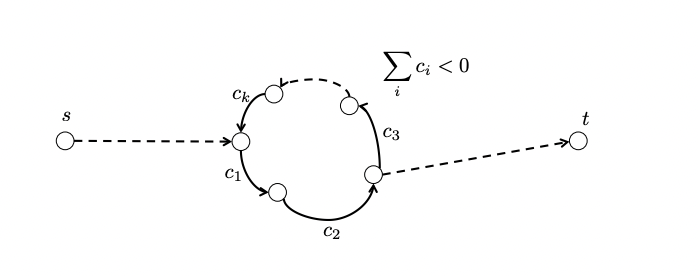
\includegraphics[scale=0.5]{negative_cycle.png}
\caption{Assume there is a negative cycle along the $s-t$ path. The distance between $s$ and
$t$ is not well-defined.}
\label{fig:negative_cycle}
\end{figure}

For example, consider the graph in Figure \ref{fig:negative_cycle}. The shortest path from $s$ to $t$ would start from the node $s$, loop around the negative cycle an infinite number of times and eventually reach destination $t$. The shortest path would, hence, be of infinite length and is not well-defined. Besides the negative cycles, there are no problems in computing the shortest paths in a graph with negative edge weights. In fact, there are many applications where allowing negative edge weights is important.


\section{Amortized Time}
Let's return to the Fibonacci heaps that we only very briefly mentioned above.

Note the runtimes listed for the operations of Fibonacci heaps are not worst-case runtimes.
Instead, they are, what we call amortized runtimes. We say an operation on a data structure
takes amortized $t(n)$ time if starting from an empty data structure, performing the operation
$L$ times takes $O(L × t(n))$ time in total. This means the runtime of the operation is $O(t(n))$ when averaged over the sequence of $L$ instances of the operation. Each individual operation
call may take much more than $t(n)$ time, but this is compensated by many cheap operation
calls (that take much less than $t(n)$ time).

We analyze the amortized cost of incrementing a binary counter by one when the count
is represented in binary. Consider a b-bit counter which starts at $0$ (i.e. b $0$'s). In each
increment operation, we update the counter's bits correspondingly by flipping some bits from
$0$ to $1$, or vice versa.

Some of the increment operations may take $\Omega(b)$ time. For example, an increment operation
can require carrying $b$ bits:

\begin{align*}
1111111& \\
+ 1& \\
= 10000000&
\end{align*}

Other increments may take $O(1)$ time. 
\begin{align*}
10000000& \\
+ 1& \\
=10000001& \\
\end{align*}
 
All this said, we can show the amortized cost of the increment operation on a binary counter is $O(1)$. Even though some increments take time linear in the number of bits, if we do $n$ increment operations to the counter starting from the all $0$s, each operation takes $O(1)$ time on average.

\begin{claim}{The total time to increment a binary counter $n$ times is $O(n)$} 

We use what is known as the \textit{accounting} method to prove this claim. Each nonzero bit in the binary counter will get a ``credit'' obtained from earlier increment operations that will then be used to pay for later expensive operations. More specifically, we will maintain the invariant that every $1$ in the binary representation has a ``credit'', which we represent as $\bigoplus$, associated with it. Let $x$ be the binary counter. If we start with an ``empty'' integer – that is $0$ – then clearly all $1$'s have a ``credit'' as there are no $1$'s. Assume that all the 1's of $x$ have a ``credit'' at the start of an increment operation. In each increment operation, we know the first addition will require constant work for which the addition operation will be charged with. We actually ``charge'' the addition operation two ``credit''s, represented as $\bigoplus\bigoplus$, to the new $1$ to be added:

\begin{align*}
x = 1^{\bigoplus}1^{\bigoplus}0& \\
+& \\
1^{\bigoplus \bigoplus}
\end{align*}

Now we start adding. We will maintain the invariant that any ``carry'' bit will have two $\bigoplus$ credits. For completeness, we'll call the original $1$ to be added to $x$ a ``carry'' as well. 

Now, at each point we are adding a carry bit to a bit in $x$. If the carry bit is $0$, we do nothing and stop. If the carry bit to be added to the $i$-th bit is $1$ and the $i$-th bit of $x$ is $0$ (Note $i$ starts at $0$), then one of the $\bigoplus$ credits of the carry bit is used to store $1$ in $x[i]$ and the other remains on this new 1 as $\bigoplus$:

\begin{align*}
x = 1^{\bigoplus}1^{\bigoplus}0& \\
+ 1^{\bigoplus \bigoplus} \\
= 1^{\bigoplus}1^{\bigoplus}1^{\bigoplus} &
\end{align*}
At this point, the carry for the $i + 1$-st slot is $0$ and we can stop the addition.

When the carry bit to be added to the $i$-th bit is $1$ and $x[i]$ is $1$, however, we will get a non-zero carry bit for the $i + 1$-st position. In this case, we will use one $\bigoplus$from the $1$ stored in $x[i]$ to pay for storing a $0$ in $x[i]$ (doing the carry addition), and we'll move the two $\bigoplus$ of the carry bit to the new carry bit for the $i + 1$-st position. This maintains the invariant thatall $1$s in $x$ have a credit and all carries have two credits.

For example, consider an increment operation on the binary counter $x = 0111$:

\begin{align*}
01^{\bigoplus}1^{\bigoplus}1^{\bigoplus}& \\
+1^{\bigoplus\bigoplus}&
\end{align*}

A new carry bit is formed:
\begin{align*}
&1^{\bigoplus\bigoplus}\\
=01^{\bigoplus}&1^{\bigoplus}0 
\end{align*}

A new carry bit is formed:
\begin{align*}
&1^{\bigoplus\bigoplus}\\
=0&1^{\bigoplus}00 
\end{align*}

A new carry bit is formed:
\begin{align*}
&1^{\bigoplus\bigoplus}\\
=&0000 \\
=&1^{\bigoplus}000
\end{align*}
\end{claim}

All carry propagations of additions are for free because they are paid for by the credits accumulated in previous additions of $0$'s and $1$'s. There are $O(n)$ credits overall, two for each increment operation. Thus, the total runtime is $O(n)$. The credit system allows you to pay for later long operations by depositing credits from previous short operations. Some operations are long, but over all $n$ increment operations, the total work is $O(n)$. It follows that the increment operation takes amortized $O(1)$ time.
\end{document}